\chapter{Estados, mediciones y espacios vectoriales complejos}

\lectureoverview{La mecánica cuántica comienza por cambiar lo que entendemos por estado. Primero aislamos el patrón clásico de estados y evolución determinista; después, un experimento de espín con dos resultados posibles pone de manifiesto su fracaso. La respuesta matemática es un espacio vectorial complejo dotado de vectores duales, un producto interno, una norma y ortogonalidad.}

\section{El patrón clásico: estado y evolución}

Empecemos con un sistema cerrado, al menos temporalmente aislado de todo lo demás. Aquí, la palabra \emph{sistema} es un concepto primitivo: designa el objeto cuya historia queremos predecir. Un \emph{estado} es todo lo que hay que conocer en un instante para poder hacer esa predicción. La mecánica clásica proporciona una ley que actualiza un estado y lo convierte en el siguiente.

Para la moneda abstracta más sencilla,
\begin{equation}
  \mathcal S_{\mathrm{coin}}=\{H,T\}.
\end{equation}
Una ley posible establece que no ocurre nada:
\begin{equation}
  H\longmapsto H,
  \qquad
  T\longmapsto T.
\end{equation}
Otra ley alterna los dos estados:
\begin{equation}
  H\longmapsto T,
  \qquad
  T\longmapsto H.
\end{equation}
Estos ejemplos son elementales, pero revelan la estructura de una teoría clásica:
\begin{equation}
  s(t)\longmapsto s(t+\Delta t).
\end{equation}
Una vez conocido \(s(t)\), la evolución es determinista.

Este mismo patrón se mantiene cuando el espacio de estados es continuo. Para describir una partícula que se mueve en una recta hacen falta tanto su posición como su momento,
\begin{equation}
  s=(q,p),
\end{equation}
por lo que su espacio de estados es el plano de fases. El número de estados posibles pasa a ser infinito y las ecuaciones pueden escribirse con el elegante lenguaje de los lagrangianos, los hamiltonianos y los corchetes de Poisson, pero la idea subyacente no cambia. El estado en un instante contiene lo necesario para predecir el estado en otro.

\section{Abstracción antes que visualización}

El movimiento clásico es relativamente fácil de imaginar porque sus conceptos proceden de la experiencia cotidiana. Esa ventaja desaparece cuando los objetos pertinentes son demasiado pequeños, las velocidades demasiado grandes o la dimensión del espacio de estados demasiado elevada. Nadie visualiza literalmente el movimiento de un electrón, el espacio-tiempo de cuatro dimensiones o un espacio de diez dimensiones. Esto no es una deficiencia propia de los principiantes. La intuición visual humana se formó para el mundo cotidiano tridimensional.

Incluso los casos que parecen más sencillos revelan esta limitación. Lo que llamamos una imagen de un espacio curvo bidimensional suele ser una superficie embebida en tres dimensiones. Una recta unidimensional se representa como una marca en un plano. La imagen incorpora, sin que nos demos cuenta, el espacio ambiente en el que nuestro sistema visual sabe desenvolverse.

La solución no consiste en imponer una imagen clásica a una física desconocida. Consiste en aprender la estructura abstracta y dejar que surja una intuición nueva a partir de manipulaciones correctas. Las coordenadas tridimensionales \((x,y,z)\) se convierten en coordenadas de cuatro dimensiones \((x,y,z,w)\) al añadir un símbolo y ampliar las reglas, no al adquirir un nuevo órgano de la vista. La mecánica cuántica exige la misma disciplina. Tratarla como un modelo mecánico extraño de pequeños objetos clásicos conducirá una y otra vez a respuestas equivocadas.

\begin{remark}
La intuición matemática también se desarrolla. Simplemente, no es lo mismo que ver una ola en el océano o una flecha en el espacio ordinario. El álgebra se vuelve familiar porque sus relaciones se aplican de manera coherente.
\end{remark}

\section{Espacios de estados clásicos y lógica clásica}

Para un sistema clásico, el espacio de estados es un conjunto. Un dado abstracto tiene
\begin{equation}
  \mathcal S_{\mathrm{die}}=\{1,2,3,4,5,6\}.
\end{equation}
Un dado real puede tener infinitas orientaciones, pero el dado idealizado que usamos aquí solo tiene estas seis etiquetas. Una partícula en una recta tiene el conjunto infinito continuo
\begin{equation}
  \mathcal S_{\mathrm{particle}}
  =
  \{(q,p)\mid q,p\in\mathbb R\}.
\end{equation}
Finito o infinito, cada espacio de estados clásico es una colección de posibilidades mutuamente distintas.

Una proposición sobre el sistema selecciona un subconjunto de esas posibilidades. Para el dado, sean
\begin{align}
  P_{\mathrm{odd}}&=\{1,3,5\},\\
  P_{\leq 3}&=\{1,2,3\}.
\end{align}
La afirmación \emph{impar y no mayor que tres} corresponde a su intersección:
\begin{equation}
  P_{\mathrm{odd}}\cap P_{\leq 3}=\{1,3\}.
\end{equation}
La afirmación inclusiva \emph{impar o no mayor que tres} corresponde a su unión:
\begin{equation}
  P_{\mathrm{odd}}\cup P_{\leq 3}
  =
  \{1,2,3,5\}.
\end{equation}
Así, la conjunción y la disyunción clásicas tienen la forma conjuntista
\begin{equation}
  P\wedge Q\longleftrightarrow P\cap Q,
  \qquad
  P\vee Q\longleftrightarrow P\cup Q.
\end{equation}
Si los subconjuntos no se solapan, ningún estado hace verdaderas ambas proposiciones.

Esta lógica está ligada a la concepción clásica del estado. La mecánica cuántica sustituye el conjunto de alternativas clásicas por un objeto matemático distinto: un espacio vectorial. Solo en un límite clásico adecuado la descripción mediante espacios vectoriales se comporta aproximadamente como un conjunto de configuraciones excluyentes. Antes de construir ese espacio, necesitamos un experimento que haga inevitable la sustitución.

\section{El sistema cuántico más sencillo}

El análogo cuántico de la moneda abstracta es un sistema con dos resultados posibles llamado \emph{cúbit}. Primero podemos etiquetar las alternativas medidas como cara y cruz, pero resulta más útil asignarles etiquetas numéricas:
\begin{equation}
  \sigma\in\{+1,-1\}.
\end{equation}
Usaremos en paralelo tres notaciones:
\begin{equation}
  H\longleftrightarrow \sigma=+1\longleftrightarrow\uparrow,
  \qquad
  T\longleftrightarrow \sigma=-1\longleftrightarrow\downarrow.
\end{equation}
Al principio, las flechas son solo nombres. Todavía no se ha supuesto que sean vectores geométricos ordinarios.

\begin{figure}[htbp]
  \centering
  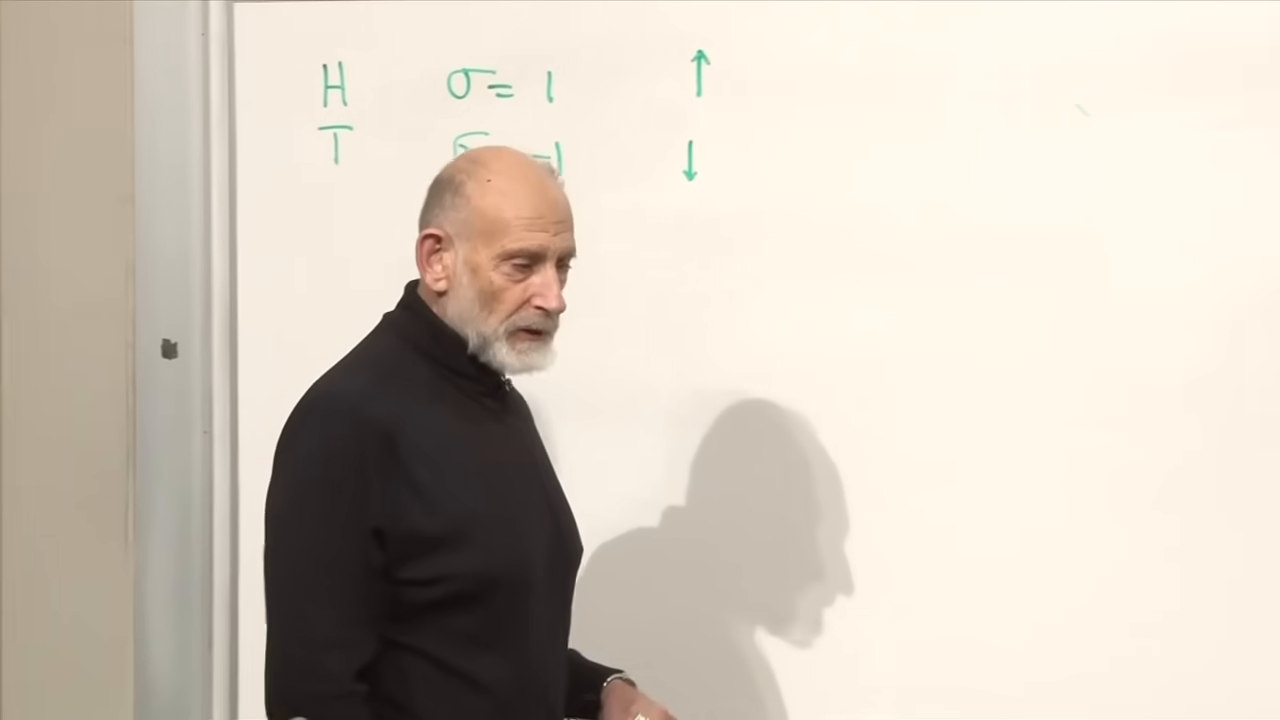
\includegraphics[width=0.78\textwidth]{lecture_01_figure_02.png}
  \caption{La pizarra presenta las etiquetas equivalentes \(H/T\), \(\sigma=\pm1\) y las flechas arriba/abajo. Al principio, las flechas son notación, no un modelo clásico.}
  \lectureframe{00:22:44}
\end{figure}

\begin{classroomqa}
\audiencequestion{¿Qué tienen que ver la cara y la cruz con el sistema físico?}
\lecturerresponse{Nada, salvo que proporcionan dos nombres conocidos. El cúbit tiene dos resultados posibles para esta medición; cara y cruz son marcadores de posición. Se eligen las etiquetas \(\pm1\) porque pueden aparecer en las ecuaciones.}
\end{classroomqa}

\subsection{El aparato como caja negra}

Un experimento requiere un segundo sistema: el aparato \(A\). Por ahora es una caja negra abstracta con tres características:
\begin{enumerate}
  \item tiene una orientación espacial, indicada por \emph{este lado hacia arriba};
  \item tiene un sensor que puede interactuar con el cúbit;
  \item tiene una pantalla que al principio está en blanco y que después muestra \(+1\) o \(-1\).
\end{enumerate}
Los detalles del detector se dejan deliberadamente para más adelante. Un buen detector se define operacionalmente por la relación fiable entre el sistema y el registro que produce. No hace falta que el observador esté mirando cuando ocurre la interacción: el aparato puede registrar el resultado y consultarse después.

Supongamos que la pantalla indica \(+1\). Reiniciemos el aparato hasta dejarlo en blanco y repitamos inmediatamente la misma medición, antes de que pueda actuar cualquier evolución independiente. Un detector fiel vuelve a indicar \(+1\). Si el primer resultado es \(-1\), las repeticiones inmediatas también siguen indicando \(-1\):
\begin{equation}
\begin{aligned}
  +1&\longrightarrow +1\longrightarrow +1\longrightarrow\cdots,\\
  -1&\longrightarrow -1\longrightarrow -1\longrightarrow\cdots.
\end{aligned}
\end{equation}
Por tanto, podemos considerar la primera medición una \emph{preparación}. Deja el cúbit en un estado en el que una repetición inmediata de la misma medición da un resultado definido.

Esta repetibilidad no es una interpretación filosófica opcional. Sin ella, no habría forma operacional de confirmar una medición. Un dispositivo defectuoso puede no repetir su resultado, pero entonces no está realizando la medición ideal que hemos definido.

\begin{classroomqa}
\audiencequestion{¿Es esto ya el colapso de la función de onda?}
\lecturerresponse{Podemos introducir ese lenguaje más adelante. Por ahora basta con la afirmación operacional: una medición produce un resultado y prepara un estado en el que la misma medición inmediata vuelve a dar ese resultado. Ponerle nombre al proceso todavía no lo explica.}
\end{classroomqa}

\section{La orientación y el fracaso del indicador clásico}

Preparemos el cúbit de modo que el aparato vertical indique \(+1\). Giremos el aparato \(180^\circ\) y repitamos la medición. Ahora el resultado es \(-1\). Las mediciones repetidas con el aparato invertido confirman \(-1\), mientras que volver a ponerlo vertical restablece \(+1\).

El resultado revela una direccionalidad real. La notación arriba/abajo no es del todo arbitraria: al invertir el detector, se invierte el signo. Resulta tentador concluir que el cúbit es simplemente un vector pequeño y que el detector mide la componente de ese vector a lo largo de su propio eje. Hay que poner a prueba esa tentación, no darla por cierta.

\begin{figure}[htbp]
  \centering
  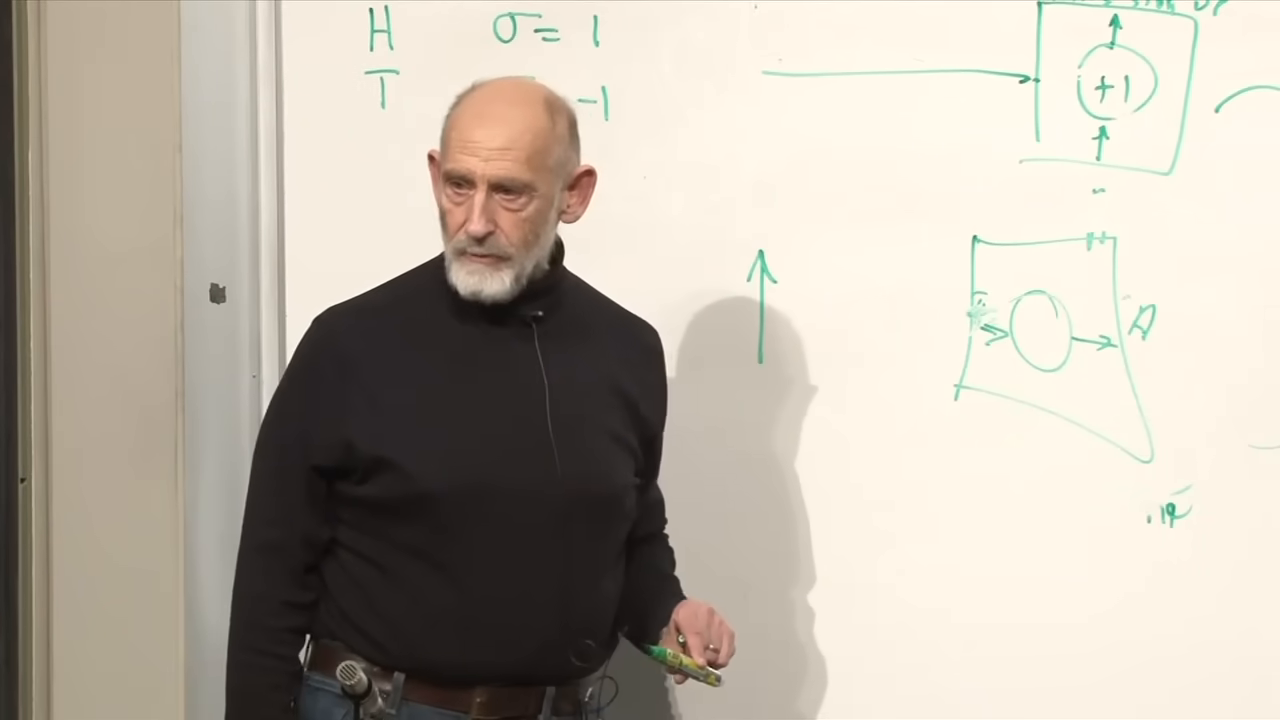
\includegraphics[width=0.82\textwidth]{lecture_01_figure_03.png}
  \caption{Una preparación hacia arriba y analizadores con distintas orientaciones en la pizarra. Más adelante, en clase se corrigió la dirección de una de las flechas de tiza; para el argumento solo importa el eje del analizador.}
  \lectureframe{00:36:21}
\end{figure}

\subsection{Una medición lateral}

Giremos el detector \(90^\circ\). Si el cúbit preparado fuera un indicador ordinario orientado hacia arriba, su componente a lo largo del eje horizontal del detector sería cero:
\begin{equation}
  \hat{\mathbf x}\cdot\hat{\mathbf z}=0.
\end{equation}
El aparato cuántico nunca indica cero. Cada ensayo individual da \(+1\) o \(-1\).

\begin{figure}[htbp]
  \centering
  \resizebox{\linewidth}{!}{%
  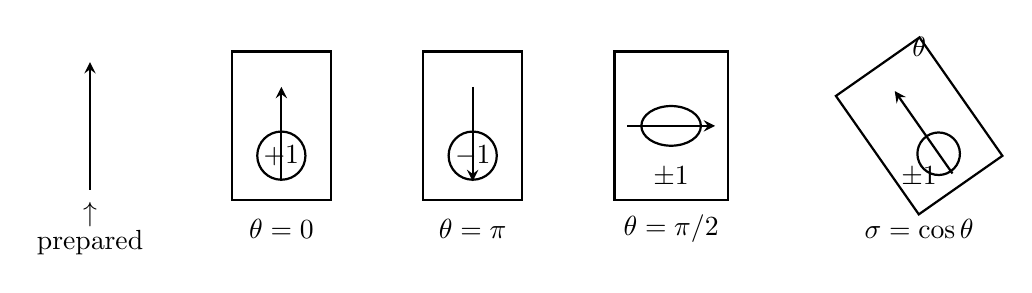
\begin{tikzpicture}[>=stealth,thick,scale=0.90]
    \draw[->] (0,0)--(0,1.8);
    \node at (0,-0.35) {\(\uparrow\)};
    \node at (0,-0.75) {prepared};

    \draw (2.0,-0.15) rectangle (3.4,1.95);
    \draw (2.7,0.48) circle (0.34);
    \draw[->] (2.7,0.12)--(2.7,1.45);
    \node at (2.7,0.48) {\(+1\)};
    \node at (2.7,-0.55) {\(\theta=0\)};

    \draw (4.7,-0.15) rectangle (6.1,1.95);
    \draw (5.4,0.48) circle (0.34);
    \draw[->] (5.4,1.45)--(5.4,0.12);
    \node at (5.4,0.48) {\(-1\)};
    \node at (5.4,-0.55) {\(\theta=\pi\)};

    \draw (7.4,-0.15) rectangle (9.0,1.95);
    \draw (8.2,0.90) ellipse (0.42 and 0.28);
    \draw[->] (7.58,0.90)--(8.82,0.90);
    \node at (8.2,0.18) {\(\pm1\)};
    \node at (8.2,-0.55) {\(\theta=\pi/2\)};

    \begin{scope}[shift={(11.7,0.90)},rotate=35]
      \draw (-0.72,-1.02) rectangle (0.72,1.02);
      \draw (0,-0.48) circle (0.30);
      \draw[->] (0,-0.82)--(0,0.60);
    \end{scope}
    \node at (11.7,0.18) {\(\pm1\)};
    \node at (11.7,-0.55) {\(\expect{\sigma}=\cos\theta\)};
    \node at (11.7,2.02) {\(\theta\)};
  \end{tikzpicture}
  }%
  \caption{Reconstrucción de la secuencia de analizadores. La rotación cambia las estadísticas, pero nunca el conjunto de resultados individuales.}
\end{figure}

Preparemos un conjunto grande de cúbits con el aparato vertical y conservemos aquellos para los que el resultado sea \(+1\). Midamos una sola vez cada cúbit conservado con el aparato lateral. La mitad de los ensayos da \(+1\) y la otra mitad \(-1\); el promedio del conjunto es cero:
\begin{equation}
  \expect{\sigma}_{\pi/2}=0.
\end{equation}
El promedio se parece a la componente horizontal nula de un indicador clásico, pero los registros individuales no. El valor clásico \(0\) ha sido sustituido por un equilibrio estadístico entre dos resultados discretos.

\begin{classroomqa}
\audiencequestion{¿Qué ocurre si se conserva el mismo cúbit en vez de descartarlo después de la medición lateral?}
\lecturerresponse{Supongamos que el primer resultado lateral es \(+1\). Si repetimos la medición lateral con ese mismo cúbit, volvemos a obtener \(+1\) una y otra vez. La primera medición lateral lo ha preparado con respecto al eje lateral. Para obtener las estadísticas de mitad y mitad, hay que repetir todo el experimento de preparación y medición con muchos cúbits, no confirmar repetidamente un único resultado.}
\end{classroomqa}

\subsection{Preparaciones incompatibles}

La secuencia de ejes importa. Preparemos \(+1\) en dirección vertical y midamos después en dirección horizontal. El primer resultado horizontal es aleatorio. Una vez obtenido, las repeticiones horizontales inmediatas dan un resultado definido. Ahora volvamos a girar el detector hasta el eje vertical. El resultado vertical vuelve a ser aleatorio.

En notación, donde \(M_z\) y \(M_x\) representan mediciones a lo largo de los dos ejes,
\begin{equation}
\begin{aligned}
  M_z&:+1,\\
  M_x&:\pm1,\\
  M_x&:\text{same result},\\
  M_z&:\pm1.
\end{aligned}
\end{equation}
La medición intermedia \(x\) no se ha limitado a revelar una componente horizontal conservando el estado vertical original. Ha preparado un estado nuevo y se ha perdido la certeza vertical original.

\begin{classroomqa}
\audiencequestion{¿El detector recuerda la primera respuesta? ¿Cómo puede saber si se le ha presentado el mismo cúbit o uno nuevo?}
\lecturerresponse{La repetibilidad es una propiedad del cúbit medido, no una comparación con una memoria oculta del detector. Después de una medición, el cúbit queda en un estado que da la misma respuesta al repetir inmediatamente esa medición. Si se presenta un cúbit preparado de otra manera, el resultado depende de esa preparación. Llevar la cuenta de qué sistema físico se está midiendo es una tarea habitual de laboratorio.}
\end{classroomqa}

\begin{classroomqa}
\audiencequestion{Entonces, ¿el acto de observar prepara ese cúbit en particular?}
\lecturerresponse{Sí. Una vez que la medición ha preparado el cúbit, la misma medición da la misma respuesta hasta que intervenga otra evolución o una medición incompatible.}
\end{classroomqa}

\section{Un analizador girado un ángulo arbitrario}

Sea \(\theta\) el ángulo entre el eje del detector y el eje a lo largo del cual se preparó el conjunto. En cada ensayo se obtiene siempre
\begin{equation}
  \sigma=\pm1.
\end{equation}
Las frecuencias relativas varían con el ángulo, de modo que la media es
\begin{equation}
  \expect{\sigma}_{\theta}=\cos\theta.
  \label{eq:qml1-cosine-mean}
\end{equation}
Los casos límite son
\begin{align}
  \expect{\sigma}_{0}&=+1,\\
  \expect{\sigma}_{\pi/2}&=0,\\
  \expect{\sigma}_{\pi}&=-1.
\end{align}
Cerca de \(\theta=0\), la mayoría de los resultados son \(+1\), con algún \(-1\) ocasional. Cerca de \(\theta=\pi\), la mayoría son \(-1\), con algún \(+1\) ocasional.

\begin{figure}[htbp]
  \centering
  \includegraphics[width=0.82\textwidth]{lecture_01_figure_04.png}
  \caption{La pizarra real para el experimento con ángulo arbitrario: un conjunto preparado verticalmente entra en un analizador inclinado \(\theta\).}
  \lectureframe{00:48:55}
\end{figure}

La magnitud suave, semejante a la de un vector, es la media del conjunto, no el resultado individual. Si \(p_+(\theta)\) y \(p_-(\theta)\) son las dos probabilidades, entonces
\begin{equation}
  p_+ + p_-=1,
  \qquad
  p_+-p_-=\cos\theta.
\end{equation}
Por consiguiente,
\begin{equation}
\begin{aligned}
  p_+(\theta)&=\frac{1+\cos\theta}{2}
  =\cos^2\frac{\theta}{2},\\
  p_-(\theta)&=\frac{1-\cos\theta}{2}
  =\sin^2\frac{\theta}{2}.
\end{aligned}
  \label{eq:qml1-half-angle-probabilities}
\end{equation}
\editorialnote{La clase enuncia los dos resultados y su media \(\cos\theta\). La ecuación~\eqref{eq:qml1-half-angle-probabilities} se deduce de inmediato algebraicamente de esas afirmaciones y explicita la ley de frecuencias implícita.}

\begin{classroomqa}
\audiencequestion{¿Un conjunto de cúbits no preparados también presentaría la media \(\cos\theta\)?}
\lecturerresponse{En un conjunto no polarizado no se ha seleccionado ninguna dirección particular, por lo que su media es cero. La dependencia respecto de \(\theta\) se refiere a un conjunto preparado primero a lo largo de un eje definido.}
\end{classroomqa}

\begin{classroomqa}
\audiencequestion{¿Por qué hace falta todo un conjunto si el cúbit no tiene dinámica entre mediciones?}
\lecturerresponse{La primera medición inclinada de un cúbit proporciona una muestra. Todas las repeticiones inmediatas con ese mismo cúbit se limitan a confirmar esa muestra. Para obtener ensayos independientes hacen falta cúbits preparados de manera idéntica, cada uno medido una sola vez con el analizador inclinado.}
\end{classroomqa}

\begin{classroomqa}
\audiencequestion{¿Hay patrones o correlaciones de orden superior en la secuencia de signos más y menos?}
\lecturerresponse{En este experimento se supone que los ensayos separados son independientes y no están correlacionados. Las probabilidades de cada ensayo dependen de \(\theta\), pero no se afirma ningún patrón adicional en el orden de los resultados.}
\end{classroomqa}

\subsection{Qué se ha idealizado}

Por ahora, el aparato se trata como un objeto clásico con una orientación ajustable continuamente y una lectura discreta. Esta distinción entre \emph{sistema} y \emph{detector} es temporal. El detector también es un sistema físico y, a la larga, debe obedecer la mecánica cuántica. Una explicación completa tratará conjuntamente el sistema y el aparato, pero para ello hacen falta herramientas que todavía no tenemos.

\begin{classroomqa}
\audiencequestion{¿Es el detector en sí otro sistema de dos estados?}
\lecturerresponse{Tiene estados físicos y, en última instancia, debe incluirse en la descripción cuántica. Por ahora mantenemos una división operacional: el cúbit es el objeto que describimos mediante la mecánica cuántica, mientras que el detector orientado proporciona un registro clásico estable. Más adelante habrá que analizar el sistema combinado como un conjunto de sistemas cuánticos que interactúan.}
\end{classroomqa}

\begin{classroomqa}
\audiencequestion{¿Cambiar el eje alrededor del cual se gira el detector introduce más estructura que el único ángulo que se muestra aquí?}
\lecturerresponse{Sí, la descripción tridimensional completa es más rica. La rotación en un plano es su versión más sencilla y es compatible con el tratamiento más completo que veremos después.}
\end{classroomqa}

\begin{classroomqa}
\audiencequestion{¿Puede el detector dar un valor continuo entre \(-1\) y \(+1\)?}
\lecturerresponse{Su orientación varía continuamente, pero cada lectura ideal del cúbit sigue siendo \(+1\) o \(-1\). Al cambiar la orientación, la continuidad aparece en las probabilidades y los promedios, no en los resultados individuales.}
\end{classroomqa}

\section{Indicadores y vectores abstractos}

Por ahora, dejemos de lado los hechos experimentales y centrémonos en las matemáticas. Llamaremos \emph{indicador} a una flecha ordinaria en el espacio físico. Un vector matemático es un concepto más general: es un elemento de un espacio vectorial y no tiene por qué apuntar en ninguna dirección del espacio ordinario.

\begin{definition}Un espacio vectorial complejo \(V\) es una colección de vectores en la que están definidas la suma de vectores y la multiplicación por escalares complejos, y estas operaciones satisfacen las reglas habituales de linealidad. En particular, para \(u,v,w\in V\) y \(a,b\in\mathbb C\),
\begin{align}
  u+v&=v+u,\\
  (u+v)+w&=u+(v+w),\\
  a(u+v)&=au+av,\\
  (a+b)u&=au+bu,\\
  (ab)u&=a(bu),\\
  1u&=u.
\end{align}
Existe un vector cero \(0\) y, para cada \(u\), un inverso aditivo \(-u\).
\end{definition}

Al principio, la explicación en clase solo destaca las operaciones y la propiedad de clausura:
\begin{equation}
\begin{aligned}
  u,v\in V&\Longrightarrow u+v\in V,\\
  a\in\mathbb C,\ u\in V&\Longrightarrow au\in V.
\end{aligned}
\end{equation}
El vector cero y la conmutatividad se añaden después, en respuesta a las preguntas. Los demás axiomas habituales explicitan lo que ya se usa al introducir el modelo concreto de vectores columna.

Los números reales forman un espacio vectorial unidimensional sobre \(\mathbb R\). Los números complejos forman un espacio vectorial unidimensional sobre \(\mathbb C\) y bidimensional sobre \(\mathbb R\). Las funciones de valores complejos \(\psi(x)\) también forman un espacio vectorial complejo, porque
\begin{equation}
  (\psi+\phi)(x)=\psi(x)+\phi(x),
  \qquad
  (z\psi)(x)=z\psi(x).
\end{equation}
Este ejemplo de espacio de funciones cobrará importancia más adelante, pero primero las columnas finitas permiten ver la estructura con mayor facilidad.

\begin{classroomqa}
\audiencequestion{¿En qué se diferencian un vector y un espacio vectorial?}
\lecturerresponse{Un vector es un elemento. Un espacio vectorial es la colección de todos esos elementos, junto con las reglas para sumarlos y multiplicarlos por escalares, del mismo modo que un número es un objeto, mientras que el sistema numérico es una colección dotada de operaciones.}
\end{classroomqa}

\section{Columnas complejas de dos componentes}

Escribamos un vector abstracto en notación de Dirac como \(\ket{\alpha}\). Una representación concreta es
\begin{equation}
  \ket{\alpha}
  \longleftrightarrow
  \begin{pmatrix}
    \alpha_1\\
    \alpha_2
  \end{pmatrix},
  \qquad
  \alpha_1,\alpha_2\in\mathbb C.
\end{equation}
Si
\begin{equation}
  \ket{\beta}
  \longleftrightarrow
  \begin{pmatrix}
    \beta_1\\
    \beta_2
  \end{pmatrix},
\end{equation}
entonces, la suma y la multiplicación por un escalar se definen componente a componente:
\begin{align}
  \ket{\alpha}+\ket{\beta}
  &\longleftrightarrow
  \begin{pmatrix}
    \alpha_1+\beta_1\\
    \alpha_2+\beta_2
  \end{pmatrix},\\
  z\ket{\alpha}
  &\longleftrightarrow
  \begin{pmatrix}
    z\alpha_1\\
    z\alpha_2
  \end{pmatrix},
  \qquad z\in\mathbb C.
\end{align}

\begin{figure}[htbp]
  \centering
  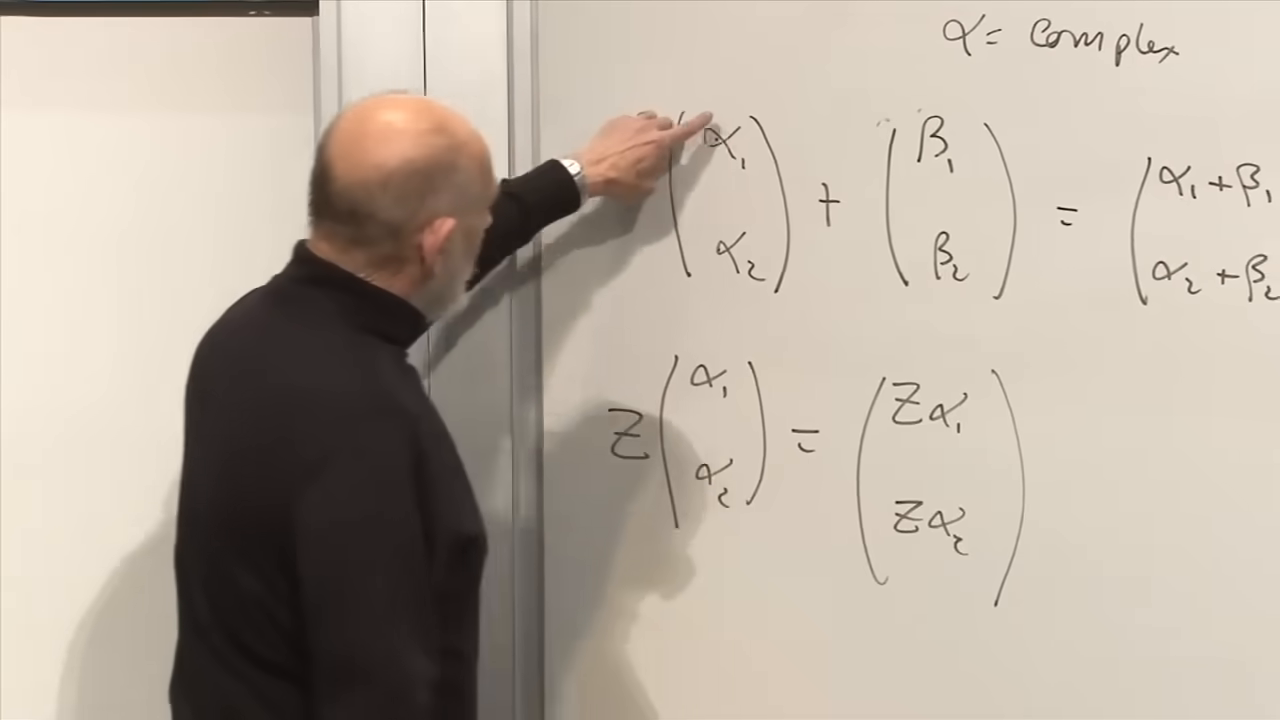
\includegraphics[width=0.88\textwidth]{lecture_01_figure_05.png}
  \caption{Las reglas componente a componente para sumar dos columnas complejas y multiplicar una columna por un escalar complejo.}
  \lectureframe{01:14:28}
\end{figure}

El vector cero es
\begin{equation}
  \ket{0}
  =
  \begin{pmatrix}
    0\\
    0
  \end{pmatrix},
  \qquad
  \ket{\alpha}+\ket{0}=\ket{\alpha}.
\end{equation}
Las columnas de longitud tres forman otro espacio vectorial, y lo mismo ocurre con cualquier longitud fija. Una columna de dos componentes no se puede sumar a una de tres: pertenecen a espacios distintos y no hay ninguna regla componente a componente que las relacione.

\begin{classroomqa}
\audiencequestion{¿Es una matriz un vector columna?}
\lecturerresponse{En la terminología general, es una matriz con una sola columna. En este curso, la palabra \emph{matriz} designará normalmente un arreglo cuadrado, mientras que un arreglo de una sola columna se llamará vector columna. La diferencia es terminológica, no una discrepancia sobre el álgebra.}
\end{classroomqa}

\begin{classroomqa}
\audiencequestion{¿Importa el orden de la suma de vectores?}
\lecturerresponse{No. La suma componente a componente hereda la conmutatividad de los números complejos:
\[
  \ket{\alpha}+\ket{\beta}
  =
  \ket{\beta}+\ket{\alpha}.
\]
Este es uno de los axiomas de los espacios vectoriales.}
\end{classroomqa}

\section{Vectores duales: bras y kets}

Para cada ket \(\ket{A}\) hay un vector correspondiente en el espacio dual, que se escribe \(\bra{A}\). La aplicación que lleva un ket a un bra es aditiva, pero conjuga los escalares complejos:
\begin{align}
  \ket{A}+\ket{B}
  &\longleftrightarrow
  \bra{A}+\bra{B},\\
  z\ket{A}
  &\longleftrightarrow
  z^*\bra{A}.
  \label{eq:qml1-antilinear-dual}
\end{align}
Esta segunda regla es la característica esencial del caso complejo. El dual de un múltiplo escalar se multiplica por el escalar complejo conjugado.

\begin{figure}[htbp]
  \centering
  \includegraphics[width=0.86\textwidth]{lecture_01_figure_06.png}
  \caption{La correspondencia de ket a bra y sus dos reglas: las sumas se transforman en sumas, mientras que la multiplicación por escalares se conjuga complejamente.}
  \lectureframe{01:23:15}
\end{figure}

Para la representación de dos componentes,
\begin{equation}
  \ket{\alpha}
  =
  \begin{pmatrix}
    \alpha_1\\
    \alpha_2
  \end{pmatrix}
  \qquad\Longrightarrow\qquad
  \bra{\alpha}
  =
  \begin{pmatrix}
    \alpha_1^*&\alpha_2^*
  \end{pmatrix}.
  \label{eq:qml1-bra-from-ket}
\end{equation}
La conjugación compleja implementa la correspondencia dual, y la notación de fila mantiene claramente diferenciados los dos tipos de objeto. La ecuación~\eqref{eq:qml1-bra-from-ket} también verifica directamente la ecuación~\eqref{eq:qml1-antilinear-dual}.

\section{El producto interno}

Dados \(\ket{\alpha}\) y \(\ket{\beta}\), combinemos el bra asociado a \(\beta\) con el ket \(\alpha\):
\begin{equation}
  \braket{\beta}{\alpha}
  =
  \begin{pmatrix}
    \beta_1^*&\beta_2^*
  \end{pmatrix}
  \begin{pmatrix}
    \alpha_1\\
    \alpha_2
  \end{pmatrix}
  =
  \beta_1^*\alpha_1+\beta_2^*\alpha_2.
  \label{eq:qml1-inner-product}
\end{equation}
La palabra \emph{corchete} se forma literalmente a partir de \emph{bra} y \emph{ket}. Este es el análogo complejo del producto escalar: se multiplican las componentes correspondientes y se suman, conjugando los números complejos del bra.

\begin{figure}[htbp]
  \centering
  \includegraphics[width=0.88\textwidth]{lecture_01_figure_07.png}
  \caption{La pizarra muestra el cálculo del producto interno \(\braket{\beta}{\alpha}\), cuyo valor es \(\beta_1^*\alpha_1+\beta_2^*\alpha_2\).}
  \lectureframe{01:31:25}
\end{figure}

Al intercambiar los vectores se obtiene
\begin{equation}
  \braket{\alpha}{\beta}
  =
  \alpha_1^*\beta_1+\alpha_2^*\beta_2
  =
  \braket{\beta}{\alpha}^{*}.
  \label{eq:qml1-conjugate-symmetry}
\end{equation}
Por tanto, en general el orden importa, pero solo cambia el resultado por conjugación compleja.

\begin{classroomqa}
\audiencequestion{¿Se podría definir un producto de vectores complejos sin conjugar uno de los lados?}
\lecturerresponse{Se puede definir una expresión bilineal de ese tipo, pero entonces el producto de un vector consigo mismo no tiene por qué ser real ni positivo. Esa no es la estructura útil en mecánica cuántica. El producto interno conjugado, o hermítico, proporciona la norma y la estructura de probabilidades que necesitaremos.}
\end{classroomqa}

\subsection{Norma y positividad}

Sustituyamos \(\beta=\alpha\) en la ecuación~\eqref{eq:qml1-inner-product}:
\begin{equation}
  \braket{\alpha}{\alpha}
  =
  \alpha_1^*\alpha_1+\alpha_2^*\alpha_2
  =
  |\alpha_1|^2+|\alpha_2|^2.
  \label{eq:qml1-norm-square}
\end{equation}
Este número es igual a su propio conjugado complejo y, por tanto, es real. Es no negativo y solo se anula para el vector cero. La longitud se define como
\begin{equation}
  \|\alpha\|
  =
  \sqrt{\braket{\alpha}{\alpha}}.
\end{equation}
Así, las componentes complejas dan lugar a una longitud real ordinaria no negativa.

\begin{figure}[htbp]
  \centering
  \includegraphics[width=0.88\textwidth]{lecture_01_figure_08.png}
  \caption{El producto interno de un vector consigo mismo en la pizarra: \(\braket{\alpha}{\alpha}=|\alpha_1|^2+|\alpha_2|^2\), la norma al cuadrado.}
  \lectureframe{01:34:40}
\end{figure}

\section{Ortogonalidad y dimensión}

Dos vectores son ortogonales cuando su producto interno se anula:
\begin{equation}
  \braket{\beta}{\alpha}=0.
  \label{eq:qml1-orthogonality}
\end{equation}
La simetría conjugada hace que esta relación no dependa del orden:
\begin{equation}
  \braket{\beta}{\alpha}=0
  \quad\Longrightarrow\quad
  \braket{\alpha}{\beta}
  =
  \braket{\beta}{\alpha}^{*}
  =0.
\end{equation}

En el espacio de dos componentes, el par ortogonal más sencillo es
\begin{equation}
  \ket{e_1}
  =
  \begin{pmatrix}
    1\\
    0
  \end{pmatrix},
  \qquad
  \ket{e_2}
  =
  \begin{pmatrix}
    0\\
    1
  \end{pmatrix},
  \qquad
  \braket{e_1}{e_2}=0.
  \label{eq:qml1-standard-basis}
\end{equation}

\begin{figure}[htbp]
  \centering
  \includegraphics[width=0.88\textwidth]{lecture_01_figure_09.png}
  \caption{La pizarra construye las columnas ortogonales estándar \((1,0)^{\mathsf T}\) y \((0,1)^{\mathsf T}\).}
  \lectureframe{01:39:50}
\end{figure}

La dimensión se puede caracterizar como el mayor número de vectores no nulos mutuamente ortogonales. En un espacio bidimensional puede haber dos vectores así, pero no un tercero. Para verlo concretamente, sea
\begin{equation}
  \ket{v}
  =
  \begin{pmatrix}
    v_1\\
    v_2
  \end{pmatrix}
\end{equation}
ortogonal a ambos vectores de la ecuación~\eqref{eq:qml1-standard-basis}. Entonces
\begin{equation}
  \braket{e_1}{v}=v_1=0,
  \qquad
  \braket{e_2}{v}=v_2=0,
\end{equation}
por lo que \(\ket{v}=\ket{0}\). No existe un tercer vector no nulo ortogonal a ambos.

\begin{classroomqa}
\audiencequestion{¿No es el vector cero ortogonal a todos los vectores, de modo que habría uno más?}
\lecturerresponse{Sí; por eso la definición debe referirse a vectores mutuamente ortogonales \emph{no nulos}. El vector cero no tiene una dirección independiente y se excluye al contar la dimensión.}
\end{classroomqa}

\begin{remark}En la representación en columnas, la dimensión es igual al número de componentes. La definición de ortogonalidad es más abstracta y no depende de haber elegido previamente unas coordenadas.
\end{remark}

\section{Otras preguntas ante la pizarra}

\begin{classroomqa}
\audiencequestion{¿Se aplica la misma estructura a un espacio vectorial de funciones?}
\lecturerresponse{Sí. Una función puede considerarse una columna cuyos elementos están indexados de manera continua \(\psi(x)\). La suma y la multiplicación por escalares se definen punto a punto. El producto interno correspondiente será una integral en vez de una suma finita; desarrollaremos esa construcción más adelante.}
\end{classroomqa}

\begin{classroomqa}
\audiencequestion{¿Multiplicar un ket por un bra produce una matriz?}
\lecturerresponse{Sí. El producto interno \(\bra{\beta}\ket{\alpha}\) contrae una fila con una columna y produce un número. Al invertir el orden, \(\ket{\alpha}\bra{\beta}\), se obtiene un producto exterior, que es una matriz cuadrada. Tanto los productos internos como los exteriores serán importantes.}
\end{classroomqa}

\begin{classroomqa}
\audiencequestion{¿La medición afecta realmente al cúbit, en vez de limitarse a revelarlo?}
\lecturerresponse{Sí. La primera medición en un eje nuevo prepara un estado nuevo; por eso, repetir esa medición confirma la respuesta, mientras que volver al eje anterior restablece la incertidumbre. Esta perturbación inevitable distingue el experimento cuántico de una medición clásica idealizada, que en principio puede hacerse con una perturbación arbitrariamente pequeña.}
\end{classroomqa}

\section{Las dos partes de la construcción}

Ahora tenemos dos partes que aún no hemos unido. La parte experimental afirma lo siguiente:
\begin{enumerate}
  \item una medición ideal de un cúbit solo puede dar los resultados \(\pm1\);
  \item repetir inmediatamente la misma medición confirma el resultado;
  \item cambiar el eje del detector cambia el estado que prepara la medición;
  \item para un conjunto preparado, un analizador inclinado un ángulo \(\theta\) tiene una media de \(\cos\theta\).
\end{enumerate}
La parte matemática afirma lo siguiente:
\begin{enumerate}
  \item los estados cuánticos se representarán mediante vectores, no mediante puntos clásicos;
  \item los vectores pertinentes forman un espacio vectorial complejo;
  \item los kets tienen bras duales, y los bras actúan de forma antilineal al multiplicarlos por escalares complejos;
  \item el producto interno hermítico define la longitud, la ortogonalidad y la dimensión.
\end{enumerate}

La siguiente tarea consiste en conectar estas dos mitades. El espacio de estados complejo bidimensional de un qubit debe reproducir la repetibilidad, la aleatoriedad y las estadísticas dependientes del ángulo del experimento del analizador. Es en esa conexión, y no en una supuesta imagen clásica oculta, donde comienza la mecánica cuántica.
